\documentclass[11pt]{article}

\usepackage[top=1in, bottom=1in, left=0.5in, right=0.5in]{geometry}
\usepackage{graphicx}
\usepackage{amssymb, amsmath, amsthm}
\usepackage{epstopdf}
\usepackage{hyperref}
\usepackage{multicol, float}
\usepackage{verbatim}
\usepackage{url}
\DeclareGraphicsRule{.tif}{png}{.png}{`convert #1 `dirname #1`/`basename #1 .tif`.png}
\renewcommand{\vec}[1]{\mathbf{#1}}

\newtheorem{theorem}{Theorem}[section]
\newtheorem{lemma}[theorem]{Lemma}
\newtheorem{proposition}[theorem]{Proposition}
\newtheorem{corollary}[theorem]{Corollary}

\newenvironment{definition}[1][Definition]{\begin{trivlist}
\item[\hskip \labelsep {\bfseries #1}]}{\end{trivlist}}
\newenvironment{example}[1][Example]{\begin{trivlist}
\item[\hskip \labelsep {\bfseries #1}]}{\end{trivlist}}
\newenvironment{remark}[1][Remark]{\begin{trivlist}
\item[\hskip \labelsep {\bfseries #1}]}{\end{trivlist}}

% headers and footers
\usepackage[english]{babel}
\usepackage[utf8]{inputenc}
\usepackage{fancyhdr}
\pagestyle{fancy}
\fancyhf{}
\rhead{Page \thepage}
\lhead{Comparison of Dimensionality Reduction techniques for Dataset X}

% raise title
\usepackage{titling}
\setlength{\droptitle}{-5em}   % This is your set screw

\title{\textbf{Comparison of Dimensionality Reduction techniques for Dataset X}}
\author{Ellango Jothimurugesan, Yilun Zhou, Roger Zou}
\date{\today}

\begin{document}
\maketitle

%%%%%%%%%%%%%%%%%%%%%%%%%%%%%%%%%%%%%%%%%%%%%%%%%%%%%%%%%%%%%%%%%%%%%%%%%%%%%%%%%%%%%%%%%%%%%%%%%%%%%%%%%%%%%%

\section*{Abstract}
We will introduce some popular dimensionality reduction methods: Principal Component Analysis (PCA), Locally Linear Embedding (LLE), and Isomap. This survey assumes familiarity with elementary linear algebra. Some preliminary concepts will be given without proof.


%\begin{multicols}{2}

%%%%%%%%%%%%%%%%%%%%%%%%%%%%%%%%%%%%%%%%%%%%%%%%%%%%%%%%%%%%%%%%%%%%%%%%%%%%%%%%%%%%%%%%%%%%%%%%%%%%%%%%%%%%%%

\section*{Preliminaries}

\subsection*{Eigenvalue Decomposition (EVD)}

We will only consider the EVD for symmetric matrices, and so will only review properties applied to matrices of this type:
\begin{definition}
\emph{(Symmetric Matrix)}
Let $A$ be a $n \times n$ matrix. Then $A$ is \textit{symmetric} if $A = A^T$.
\end{definition}

We can consider the eigenvectors and eigenvalues of symmetric matrices (and square matrices in general):
\begin{definition}
\emph{(Eigenvectors and Eigenvalues)}
Let $A$ be a $n \times n$ real matrix. A non-zero vector $\mathbf{v}$ is an \textit{eigenvector} if and only if
\[A\mathbf{v} = \lambda \mathbf{v}\]
where $\lambda$ is the corresponding (scalar) \textit{eigenvalue}.
\end{definition}
Intuitively, if we consider $A$ to be a linear map $A: \mathbf{R}^n \rightarrow \mathbf{R}^n$, then an eigenvector $\mathbf{v}$ is a vector that has its direction preserved and scaled by $\lambda$ under $A$. \\

An important result of linear algebra is the spectral theorem, which formally states that:
\begin{theorem}
\emph{(Spectral Theorem and EVD)}
\label{EVD}
Let $A$ be a $n \times n$ real, symmetric matrix. Then there exists exactly $n$ eigenvalues (not necessarily distinct) $\lambda_1, \ldots, \lambda_n$, with corresponding eigenvectors $\mathbf{v}_1, \ldots, \mathbf{v}_n$ that form an orthonormal basis. Furthermore, there exists the decomposition:
\[A = Q \Lambda Q^T\]
where $Q$ is an orthogonal matrix with columns $\mathbf{v}_1, \ldots, \mathbf{v}_n$, and $\Lambda$ is a diagonal matrix with $\lambda_1, \ldots, \lambda_n$ along the diagonal.
\end{theorem}

\subsection*{Singular Value Decomposition (SVD)}

We can perform a related, extremely useful, factorization to any real $m \times n$ matrix:
\begin{theorem}
\emph{(Existence of SVD)}
\label{SVD}
Let $A$ be a real $m \times n$ matrix. Then there exists orthogonal matrices
\[U =\begin{bmatrix} \mathbf{u}_1& \ldots & \mathbf{u}_m \end{bmatrix} \qquad V =\begin{bmatrix} \mathbf{v}_1& \ldots & \mathbf{v}_n \end{bmatrix}\]
with $\mathbf{u}_i \in \mathbb{R}^m$ and $\mathbf{v}_j \in \mathbb{R}^n$, s.t.
\[A = U \Sigma V^T\]
where $\Sigma$ is a diagonal matrix with singular values $\sigma_1 \ge \ldots \ge \sigma_r \ge 0$ along the diagonal, $\mathbf{u}_1, \ldots, \mathbf{u}_m$ are the left singular vectors, and $\mathbf{v}_1, \ldots, \mathbf{v}_n$ are the right singular vectors.
\end{theorem}

This is closely related to the EVD. Indeed, it is useful to observe that:
Given $A = U\Sigma V^T$, we have that:
\begin{align*}
AA^T &= (U \Sigma V^T) (U \Sigma V^T)^T = U \Sigma^2 U^T\\
A^TA &= (U \Sigma V^T)^T (U \Sigma V^T) = V \Sigma^2 V^T
\end{align*}
Therefore, we can see that
\begin{enumerate}
\item The square of the singular values of $A$ are the eigenvalues of the symmetric $n \times n$ matrix $A^TA$ or $AA^T$.
\item The left singular vectors of $A$ are the eigenvectors of $AA^T$.
\item The right singular vectors of $A$ are the eigenvectors of $A^TA$.
\end{enumerate}

\section*{Dimensionality reduction for linear manifolds}

We are now ready to introduce the first technique that can be used for dimensionality reduction. We assume that the data lies in some $k$-dimensional approximately linear manifold in a larger $m$-dimensional vector space $\mathbb{R}^m$. The goal of dimensionality reduction is to re-express the data in $k$ necessary dimensions, rather than the much larger $m$ original dimensions. Two fundamentally related methods fall under this category: PCA and MDS. Both methods are very efficient (requiring only matrix operations and factorizations) because they exploit the linearity assumption.

\subsection*{Principal Component Analysis (PCA)}

Let $X$ be a zero-meaned $m \times n$ data matrix, where $m$ is the dimension of the data, and $n$ the number of samples.

\begin{definition}
\emph{(Covariance matrix)}
\label{Cov}
We define the covariance matrix of $X$ to be
\[C_X = \frac{1}{n-1} XX^T\]
 to be a symmetric, $m \times m$ matrix that quantifies the pairwise correlations between all data dimensions.
\end{definition}

The intuition behind PCA is to find some orthonormal basis $\mathbf{p}_1, \ldots, \mathbf{p}_m$ in $\mathbb{R}^m$ that transforms the data in the standard basis with coefficients in $X$ to this special basis represented by coefficients in $Y$ such that the covariance matrix of $Y$, $C_Y$ is diagonalized. \\

In other words, we wish to find some matrix $P$ where
\[Y = PX\]
such that the covariance matrix of $Y$,
\[C_Y = \frac{1}{n-1} YY^T\]
is diagonalized. Furthermore, the \textit{rows} $\mathbf{p}_1, \ldots, \mathbf{p}_m$ in $\mathbb{R}^m$ of $P$ are exactly the basis vectors we're looking for. This can be seen easily by considering
\[y_i = \sum_{j=1}^m \mathbf{p}_j^T \mathbf{x}_i \]

Therefore, the goal of PCA is to find $P$. \\

\begin{theorem}
\emph{(PCA)}
\label{PCA}
Let $X$ and $Y$ be a $m \times n$ matrix, where $C_Y$ is diagonalized, and let $X = U \Sigma V^T$ be the singular value decomposition of $X$. Then the matrix $P$ s.t. $Y = PX$ is
\[P = U^T\]
\end{theorem}
\begin{proof}
Let $C_Y = \frac{1}{n-1}YY^T$ be the covariance matrix of $Y$. We wish to find the $P$ s.t. $C_Y$ is diagonal.
\begin{align*}
C_Y &= \frac{1}{n-1}YY^T \\
&= \frac{1}{n-1} (PX)(PX)^T \\
&= \frac{1}{n-1} P(XX^T)P^T
\end{align*}
Taking the SVD of $X$, we have
\begin{align*}
&= \frac{1}{n-1} P(U \Sigma V^T)(U \Sigma V^T)^TP^T \\
&= \frac{1}{n-1} P (U \Sigma^2 U^T) P^T
\end{align*}
Here we make the observation that if $P = U^T$, we have by substituting that
\begin{align*}
C_Y &= \frac{1}{n-1} U^TU \Sigma^2 U^TU \\
&= \frac{1}{n-1} \Sigma^2 \\
&= \frac{1}{n-1} \begin{bmatrix} \sigma_1^2 & & \\ & \sigma_2^2 & \\ & & \ddots \end{bmatrix}
\end{align*}
This completes the proof.
\end{proof}

We now also derived a simple algorithm to compute PCA of the matrix $X$:
\begin{enumerate}
\item Take the SVD of $X = U \Sigma V^T$;
\item return $Y = U^TX$.
\end{enumerate}
This, $Y$ is a $m \times n$ matrix of the transformed data into a more ``natural'' basis (i.e. $C_Y$ is diagonalized).

\subsubsection*{PCA for dimensionality reduction}
A consequence of the eigenvalue decomposition above is that there is a natural ordering to the singular values.
\[\sigma_1 \ge \ldots \sigma_r \ge \sigma_{r+1} = \ldots = \sigma_{m}\]

Since they correspond to variances in each principal direction $\mathbf{p}_i$, if we wish to find the first three principal components (i.e. to have data in $\mathbb{R}^3$), let
\[P_3 = \begin{bmatrix} \mathbf{p}_1^T \\[0.5em] \mathbf{p}_2^T \\[0.5em] \mathbf{p}_3^T \end{bmatrix}\]
be a $3 \times m$ matrix. Then
\[Y_3 = P_3X\]
returns a $3 \times n$ data matrix $Y_3$, with n samples in the 3 principal dimensions that account for the most variance.

\subsection*{Classical Multidimensional Scaling (CMDS)}

Given some distance matrix $D$, where $d_{ij}$ measures the dissimilarity between elements $i$ and $j$, MDS attempts to find a specified low-dimensional representation that preserves distances as much as possible. Suppose $X$ is some (possibly unknown) $m \times n$ data matrix of $m$ dimensions and $n$ samples that generated $D$. Furthermore, there is a $k$-dimensional manifold embedded in $X$, which we wish to represent with $Y$. For simplicity we will measure distances with the Euclidean Metric.

\begin{theorem}
\emph{(CMDS)}
\label{CMDS}
Let $D$ be a real, symmetric $n \times n$ dissimilarity/distance matrix generated with a Euclidean metric from $X$, an unknown $m \times n$ data matrix of $n$ samples and $m$ dimensions. If $D=V \Sigma^2 V^T$ is the eigenvalue decomposition of $D$ and $\Sigma_m$ is the first $m$ rows of $\Sigma$, then
\[X = \Sigma_m V^T\]
not necessarily unique.
\end{theorem}
\begin{proof}
Let $x_i$ be the $i$-th $m$-dimensional element of $X$. Then the euclidean distance between $x_i$ and $x_j$ is:
\[d_{ij} = \| \mathbf{x}_i - \mathbf{x}_j \|_2^2\]
Writing out the terms, we have that
\[d_{ij} = \|\mathbf{x}_i\|_2^2 + \|\mathbf{x}_j\|_2^2 - 2 \mathbf{x}_i^T\mathbf{x}_j\]
For convenience, we can center and rescale $d_{ij}$. These are acceptable, linear operations on the space that imply the non-uniqueness of $X$.
\[\tilde d_{ij} = -\frac{1}{2} \left( d_{ij} - \|\mathbf{x}_i\|_2^2 - \|\mathbf{x}_j\|_2^2 \right) = \mathbf{x}_i^T\mathbf{x}_j \]
Let $\tilde D$ be the centered and rescaled distance matrix. Then we can represent in matrix notation:
\[\tilde D = X^TX\]
Since $\tilde D$ is symmetric, we can take its eigenvalue decomposition to get:
\begin{align*}
\tilde D &= V \Lambda V^T \\
&= V \Sigma^2 V^T \\
&= (V \Sigma ) (\Sigma V^T) \\
&= (\Sigma V^T)^T (\Sigma V^T)
\end{align*}
Therefore,
\[X = \Sigma V^T\]
But since $X$ is assumed to be embedded in $m$ dimensional space, we can select the first $m$ rows of $\Sigma$ $(\Sigma_m)$. So, instead
\[X = \Sigma_m V^T\]
The non-uniqueness of $X$ can be explicitly showed by the fact that for some orthogonal matrix $Q$,
\[\hat X = QX\]
also satisfies the necessary and sufficient condition
\[D = X^TX = (QX)^T(QX) = X^TQ^TQX = \hat X^T\hat X \]
This completes the proof.
\end{proof}

\subsubsection*{CMDS for dimensionality reduction}
But assuming there is a $k$-dimensional approximately linear manifold in $X$, we can reconstruct it by taking the first $k$ rows of $\Sigma$ instead of the first $m$. We now have a simple procedure to compute the CMDS of $D$ for $k << m$ dimensions:
\begin{enumerate}
\item Compute the centered, rescaled $\tilde D$ from the original $D$.
\item Take the EVD of $D = V \Sigma^2 V^T$
\item Select the first $k$ singular values in $\Sigma$, i.e. in MATLAB notation....
\[\tilde \Sigma = \Sigma(1:k, :)\]
\item return $Y = \tilde \Sigma V^T$.
\end{enumerate}
Note $Y$ is a $k \times n$ reconstructed data matrix of $n$ samples in $k$ dimensions, as desired.

\section*{Dimension reduction for non-linear manifolds}
PCA and MDS are simple and efficient methods of dimensionality reduction. They are guaranteed to find data structure that lie on a linear subspace of the input data that lie in the originally high-dimensional vector space. However, these methods fail when the structure takes the form of a nonlinear manifold (generalization of a surface to higher dimensions). One popular toy example is the ``swiss roll". Here we introduce two techniques that attempts to address these issues: Isomap and Locally Linear Embedding (LLE).

\begin{figure}[H]
\centering
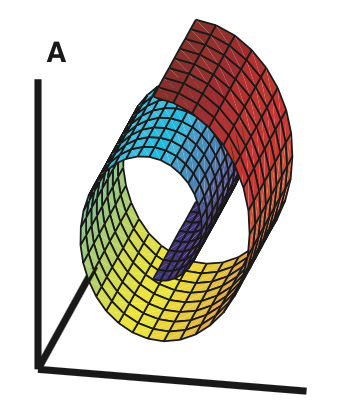
\includegraphics[width=4cm]{swissroll.png}
\caption{(From Roweis, 2000) The ``swiss roll".}
\end{figure}

\subsection*{Isomap}

Recall that Classical MDS (CMDS) finds an embedding that preserves the pairwise distances between data points, and only require a similarity ``metric" matrix $D$ as input. Isomap extends CMDS by producing $D$ that accurately represents the metric on the possibly nonlinear manifold. \\

\begin{figure}[H]
\centering
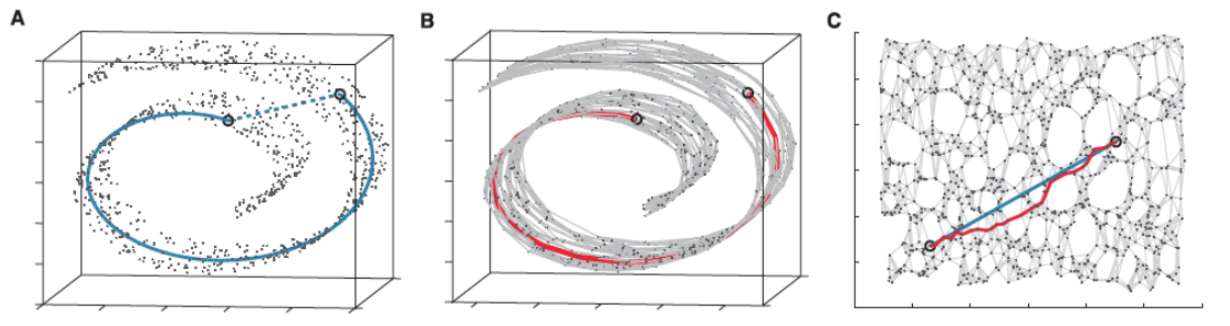
\includegraphics[width=9cm]{isomap.png}
\caption{(From Tenenbaum, 2000) True geodesic distances between points on nonlinear manifold are approximated using Isomap.}
\end{figure}

To do so, for each point $p$, Isomap utilizes some neighborhood of points $\mathcal{N}(p)$, and connects $p$ with $q \in \mathcal{N}(p)$ by an edge, with the edge cost represented by the distance between $p$ and $q$, possibly by an euclidean metric. By performing this procedure for all data points, we construct a graph $G = (V,E)$. Each entry $d_{ij}$ of $D$ is now the length of the shortest path between vertex $i$ and $j$. To compute $d_{ij}$ for all $i$ and $j$, there are efficient all-pairs shortest paths algorithms such as the Floyd-Warshall algorithm, $O(|V|^3)$. The dissimilarity/distance matrix $D$ now becomes input to classical MDS. To summarize:

\begin{enumerate}
\item define some neighborhood measure $\mathcal{N}$: for each point/vertex $p$, for all $q \in \mathcal{N}(p)$, create edge $e(p,q)$. This forms undirected graph $G = (V,E)$.
\item compute all-pairs shortest paths on $G$. The output constructs the dissimilarity matrix $D$.
\item compute Classical MDS on $D$.
\end{enumerate}

\subsection*{Locally Linear Embedding (LLE)}
This method takes a different, but intuitive approach: Although the data, globally, may lie on some nonlinear manifold, a reasonable assumption is that the data, locally, is approximately linear. \\

\begin{figure}[H]
\centering
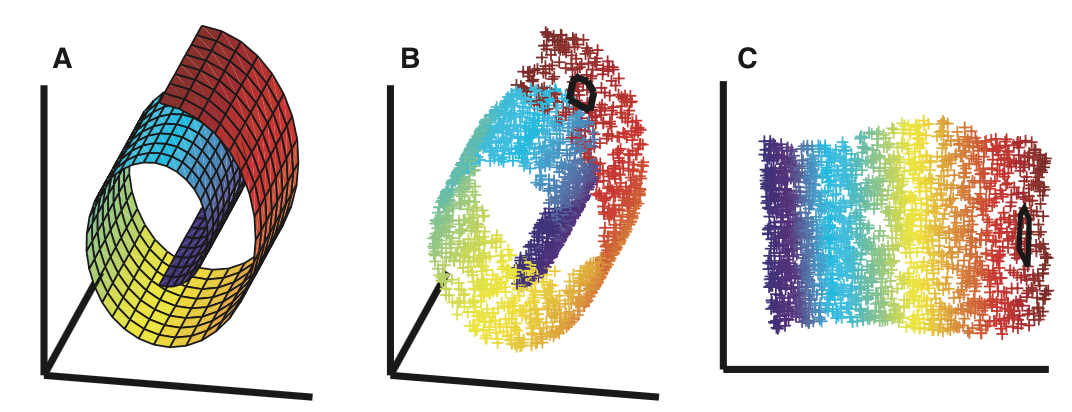
\includegraphics[width=9cm]{lle.png}
\caption{(From Roweis, 2000) The embedded lower-dimensional, non-linear manifold in high-dimensional space is detected with LLE.}
\end{figure}

\subsubsection*{Determining local weights}
The first step of LLE is to solve the local problem. Given $n$ data points in $\mathbb{R}^m$, let $\mathbf{x}_i$ be the $i^{th}$ data point and $w_{j,i}$ be the scalar weight that represents the contribution of the $j^{th}$ data point to the $i^{th}$ reconstruction. Thus it has non-zero entries if some $\mathbf{x}_j$ is a neighbor of $\mathbf{x}_i$. Let $\mathcal{N}(i)$ be the set of neighbors to $\mathbf{x}_i$. To find the best weights, we wish to solve the following constrained, least squares problem:
\[
\min_{w_{j,i}} \; \frac{1}{2} \| \mathbf{x}_i - \sum_{j \in \mathcal{N}(i)} w_{j,i}\mathbf{x}_j \|_2^2 \quad \text{s.t.} \quad  \sum_{j \in \mathcal{N}(i)}w_{j,i} = 1 \\
\]

\subsubsection*{Global reconstruction}
Given that weights are computed for each $\mathbf{x}_i$, we wish to find $\mathbf{y}_i$, the lower dimensional analog for each $\mathbf{x}_i$, by solving the following global minimization problem over all $i$.
\[\min_{\mathbf{y}_1, \ldots \mathbf{y}_n} \sum_{i=1}^n \| \mathbf{y}_i - \sum_{j \in \mathcal{N}(i)} w_{j,i} \mathbf{y}_j \| ^2 \]

\section*{Experiment on Handwritten Digit}
In this section we present results on applying dimensionality reduction to handwritten digit data. The data is in the format of $28\times 28$ pixel grey-scale image with each pixel represented by an integer by 0 to 255. The data are downloaded from \url{http://cis.jhu.edu/~sachin/digit/digit.html}. In the dataset, there are 1000 images for each digit between 0 to 9. Figure \ref{digit-vis} shows an example image of each digit.
\begin{figure}[H]
\begin{center}
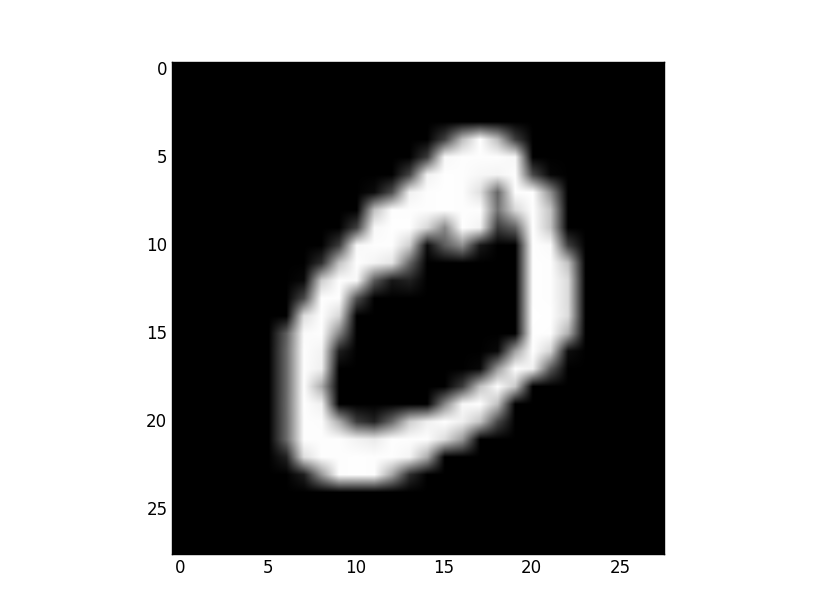
\includegraphics[width=1in]{0.png}
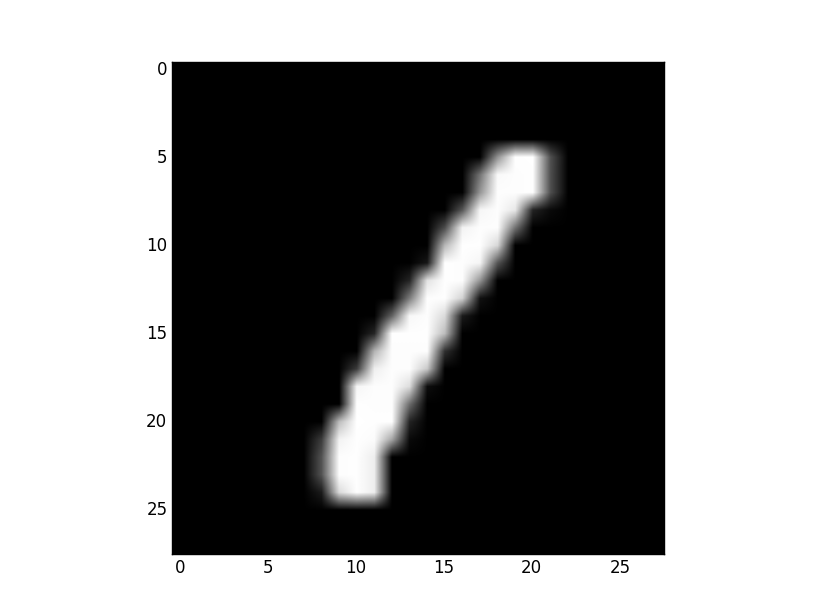
\includegraphics[width=1in]{1.png}
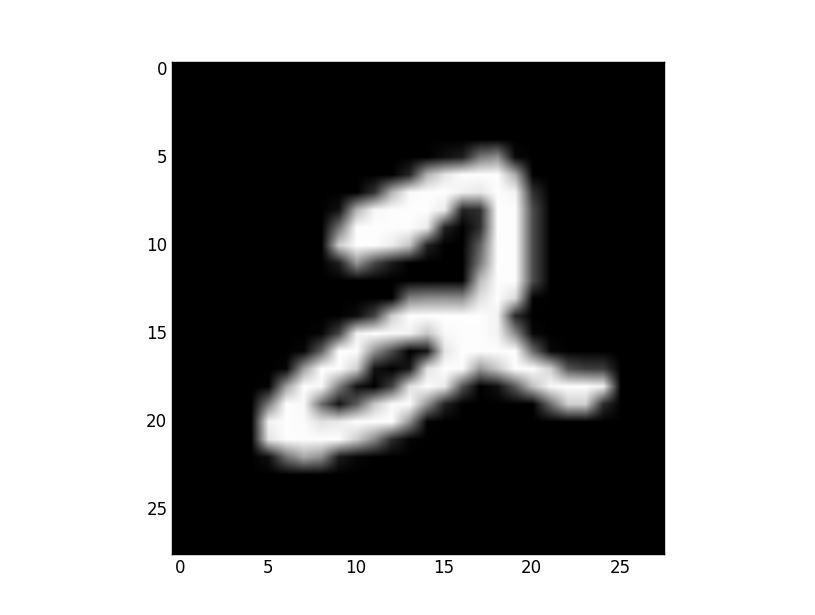
\includegraphics[width=1in]{2.png}\\
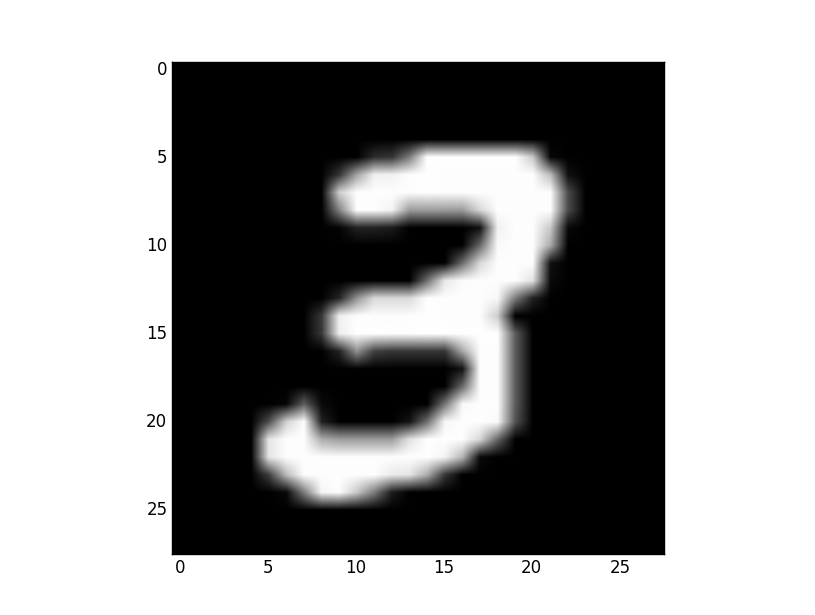
\includegraphics[width=1in]{3.png}
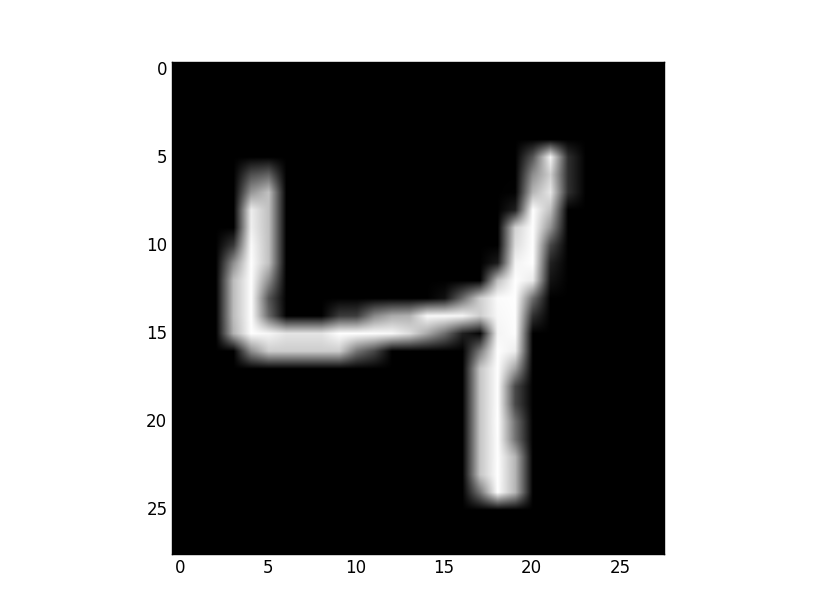
\includegraphics[width=1in]{4.png}
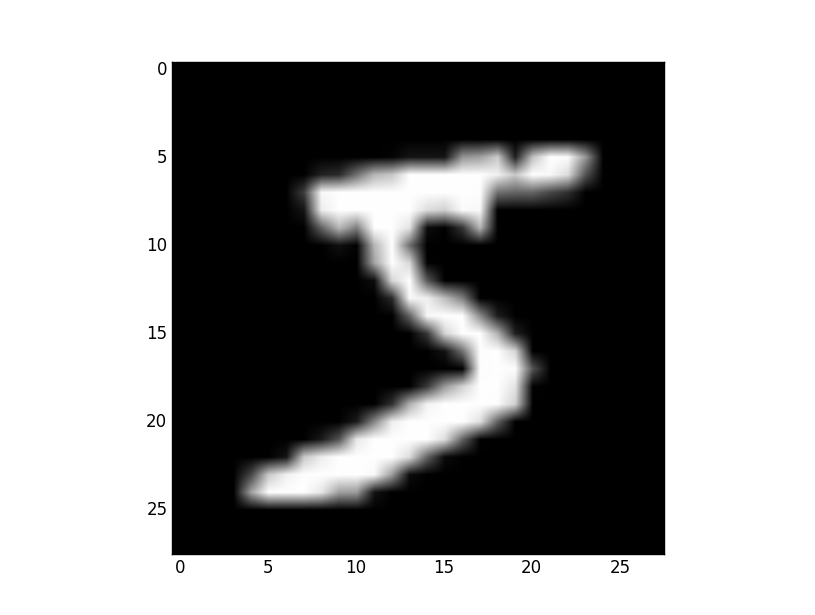
\includegraphics[width=1in]{5.png}\\
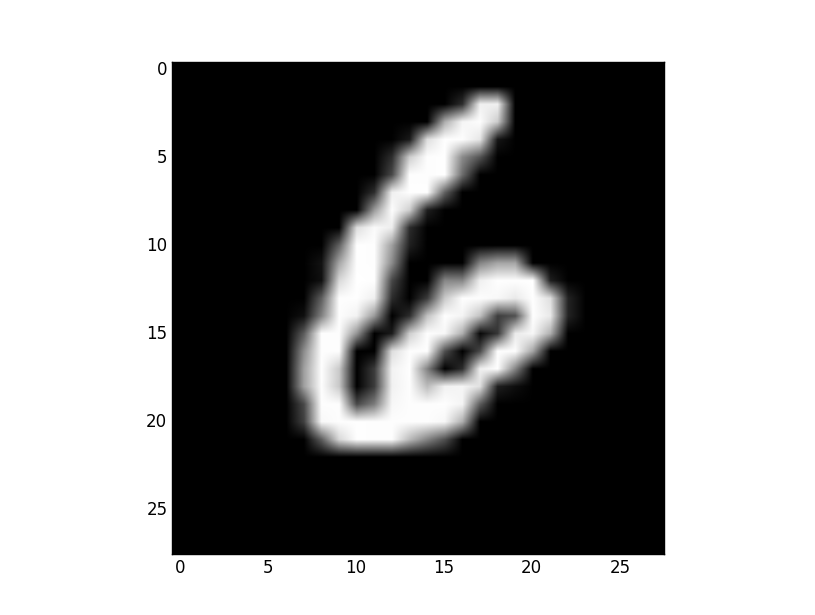
\includegraphics[width=1in]{6.png}
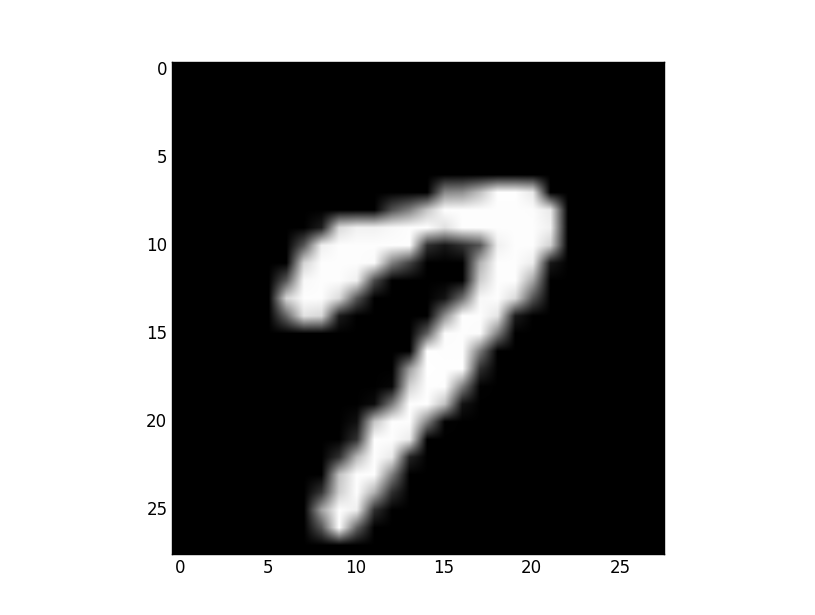
\includegraphics[width=1in]{7.png}
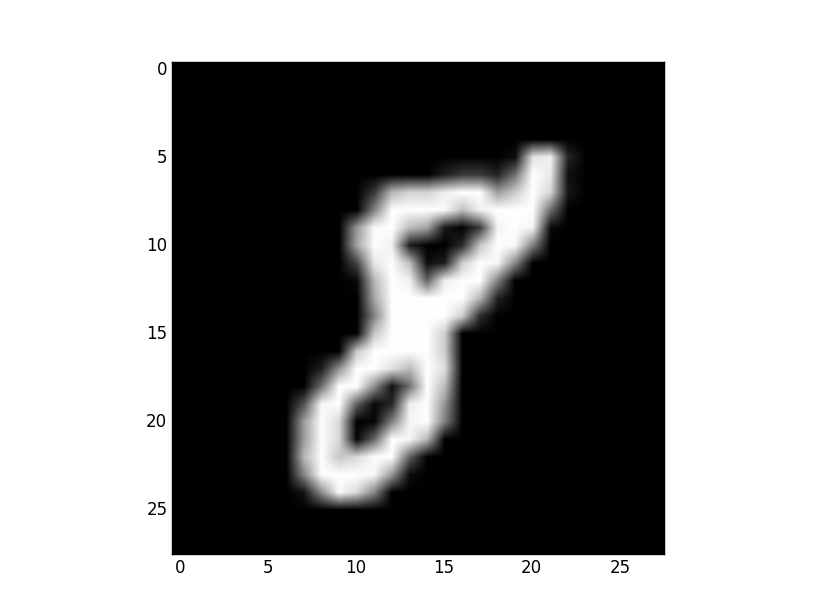
\includegraphics[width=1in]{8.png}\\
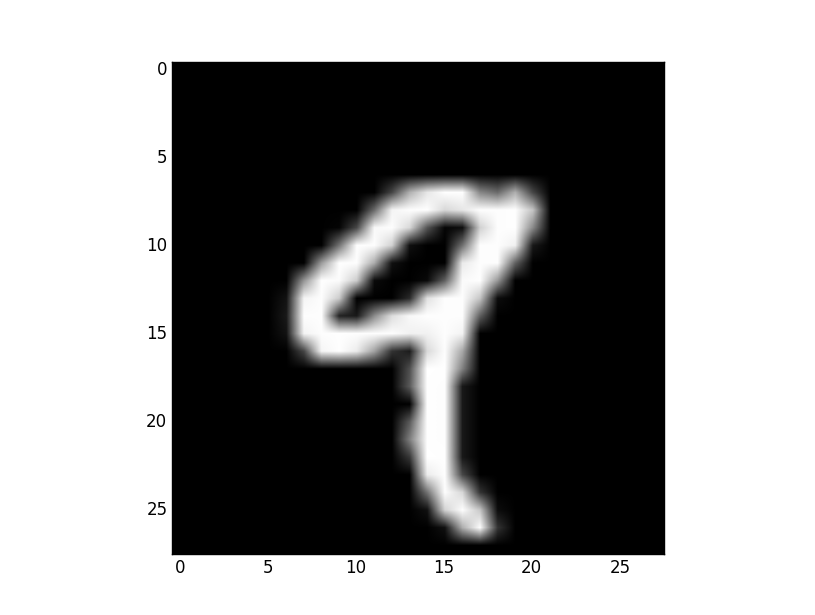
\includegraphics[width=1in]{9.png}
\caption{Visualization of digit data}
\label{digit-vis}
\end{center}
\end{figure}
When analyzing the data, we treat each image as a 784 dimensional vector.
\subsection*{Visualization Using Principal Component Analysis}
Principal component analysis is good for visualizing high dimensional data. We represent each 784-dimensional data point using two and three principal components. Figure \ref{pca_all} shows the representation of all digits, using the principal components derived from the whole dataset.
\begin{figure}[H]
\begin{center}
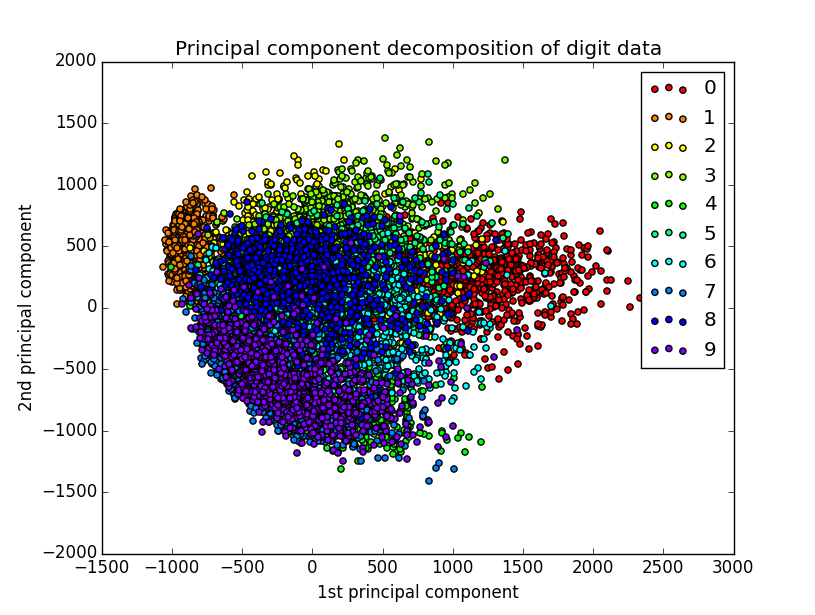
\includegraphics[width=3in]{pca_all.png}\\
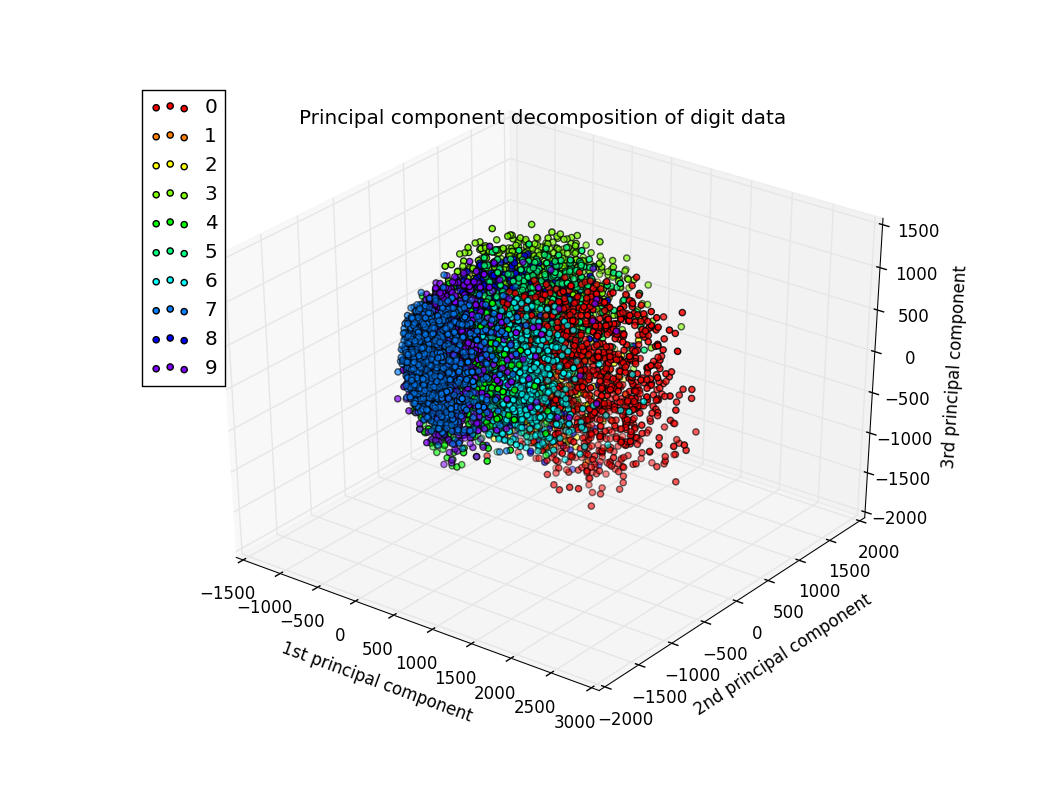
\includegraphics[width=3in]{pca_all_3d.png}
\caption{Projection of each data point onto first two and three principal components}
\label{pca_all}
\end{center}
\end{figure}
We can see that for 2D decomposition, approximate clustering effect is shown but data representing different digits still blend with each other. However, this is alleviated if we add a third principal component. Although the data representing each digit are not linearly separable, they indeed show very strong clustering effect. Thus, PCA captures the similarity between data representing same digit well. To better visualize this effect, Figure \ref{pca_012} shows projection of digit 0, 1, and 2 onto first two principal components derived from data of digit 0, 1, 2 only. We can see that data of each digit are clearly separable with only two principal components.
\begin{figure}[H]
\begin{center}
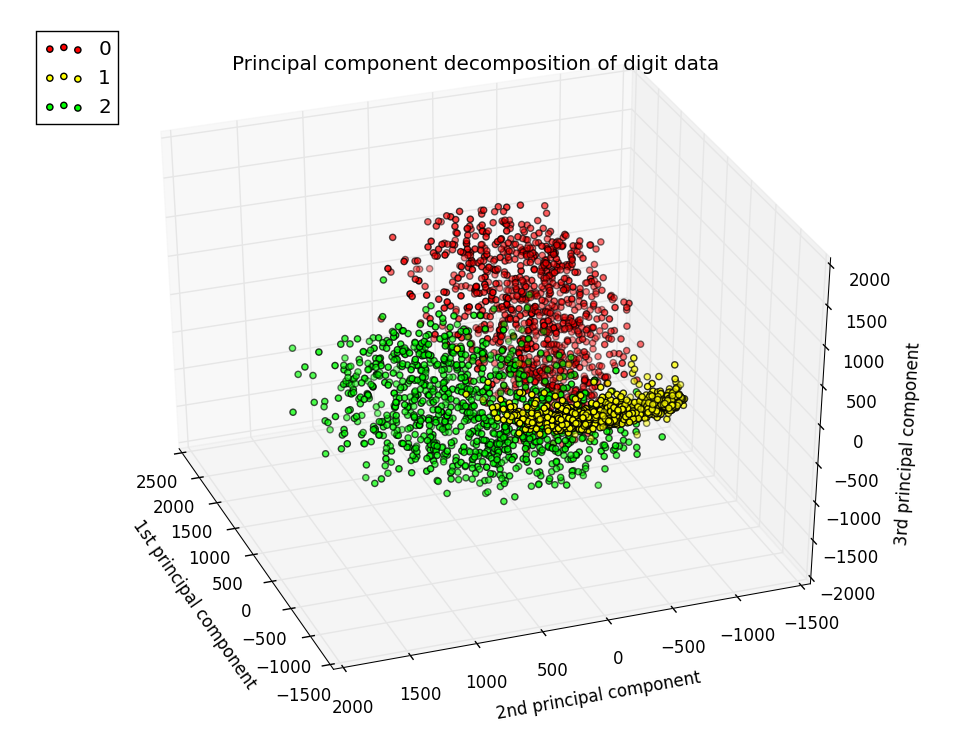
\includegraphics[width=3in]{pca_012.png}
\caption{Projection of data point for digit 0, 1, 2 onto first two principal components}
\label{pca_012}
\end{center}
\end{figure}

\subsection*{Classification Using Principal Component Analysis}
In this section we train a support vector machine (SVM) classifier to classify digit data. For 1000 data for each digit, we use 800 data for training and 200 data for testing. The feature space consists of first four principal component decompositions. We used three different classification methods: k-nearest neighbor (kNN), logistic regression, and support vector machine (SVM). for kNN, the optimal value of $k$ is selected by measuring performance on the test data. There are no free parameters in logistic regression without regularization. For SVM, we use a linear function as kernel. All three methods are implemented using \tt scikit-learn \rm library. The performance of using different number of nearest neighbors is plotted in Figure \ref{pca-knn-validation}. Table \ref{pca-error-rate} summarizes the error rate of each predictor. We see that the error rate is generally quite high. This is in part due to the fact that only four principal components are used. As shown in Figure \ref{pca-variance-explained}, four principal components can only explain 29\% variance of the data. 
\begin{figure}[H]
\begin{center}
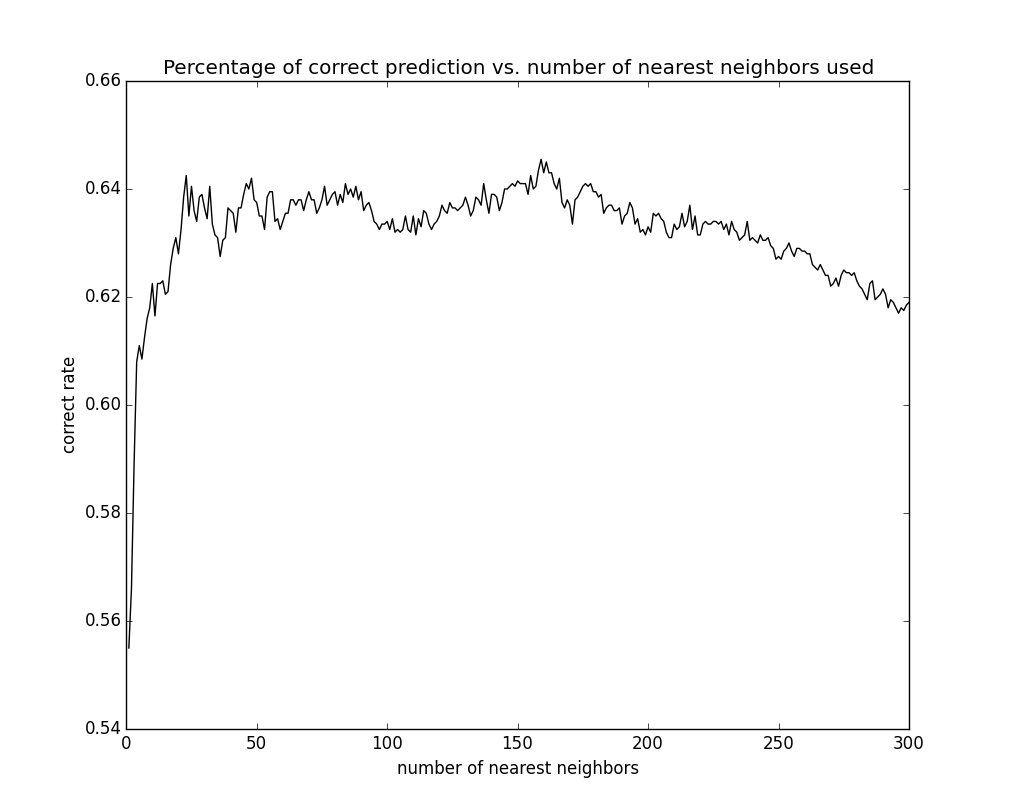
\includegraphics[width=3in]{pca-knn.png}
\end{center}
\caption{Performance of kNN classifier with different number of neighbors}
\label{pca-knn-validation}
\end{figure}
\begin{table}[H]
\begin{center}
\begin{tabular}{|c|c|c|}\hline
kNN & logistic & SVM\\\hline
0.3545 & 0.452 & 0.7865 \\\hline
\end{tabular}
\end{center}
\caption{Error rate for different classification algorithms using PCA as dimensionality reduction}
\label{pca-error-rate}
\end{table}
\begin{figure}[H]
\begin{center}
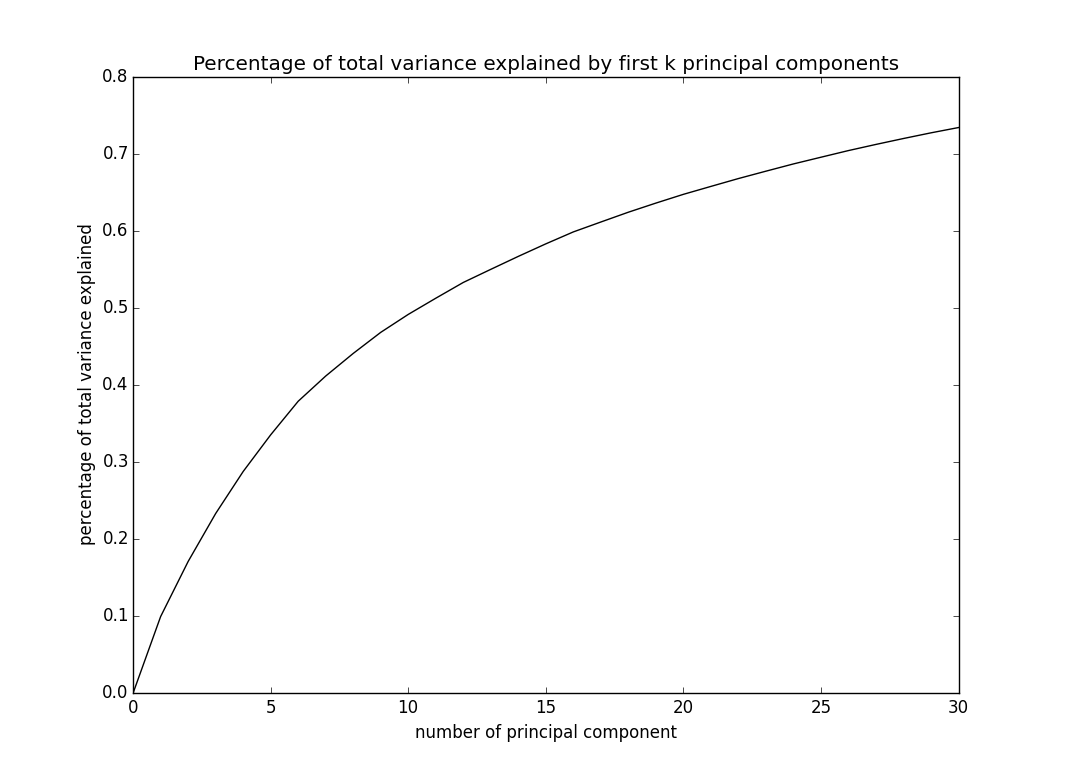
\includegraphics[width=3in]{pca_explained.png}
\end{center}
\caption{Percentage of variance explained by principal components}
\label{pca-variance-explained}
\end{figure}


%%%%%%%%%%%%%%%%%%%%%%%%%%%%%%%%%%%%%%%%%%%%%%%%%%%%%%%%%%%%%%%%%%%%%%%%%%%%%%%%%%%%%%%%%%%%%%%%%%%%%%%%%%%%%%

\section*{References}
\mbox{} \\
Roweis, S. T., \& Saul, L. K. (2000). Nonlinear dimensionality reduction by locally linear embedding. Science, 290(5500), 2323-2326. \\
\mbox{} \\
Tenenbaum, J. B., De Silva, V., \& Langford, J. C. (2000). A global geometric framework for nonlinear dimensionality reduction. Science, 290(5500), 2319-2323. \\
\mbox{} \\
Tomasi, C. Accessed 2015. Orthogonal Matrices and the Singular Value Decomposition.\\
https://www.cs.duke.edu/courses/fall13/compsci527/ notes/svd.pdf \\
\mbox{} \\
Accessed 2015. Other Dimension Reduction Techniques. \\
http://www.stat.cmu.edu/~ryantibs/advmethods/notes/ otherdr.pdf \\
\mbox{} \\


%\end{multicols}

\end{document}
